% Color Picker の手動確認用サンプル (pdflatex)。
% 1 ページ目は page 座標 (pt, 左下原点) を決め打ちした「テストボード」。
% 期待値は README.md の表を参照。
\documentclass[a4paper,11pt]{article}
\usepackage[margin=25mm]{geometry}
\usepackage[dvipsnames]{xcolor}
\usepackage{tikz}
\usetikzlibrary{patterns}
\usepackage{graphicx}
\usepackage{spotxcolor}
\pagestyle{empty}

\definecolor{cmykred}{cmyk}{0,1,1,0}
\definecolor{rgbblue}{rgb}{0,0.4,1}
\definecolor{gray50}{gray}{0.5}
\definecolor{richblack}{cmyk}{0.6,0.4,0.4,1}
\definespotcolor{DIC161s}{DIC 161s*}{0, 0.64, 1, 0}

\begin{document}

% ---------------------------------------------------------------- page 1
\noindent
Plain body text (DeviceGray 0).\quad
\textcolor{cmykred}{CMYK red text.}\quad
\textcolor{rgbblue}{RGB blue text.}\quad
\textcolor{gray50}{Gray 50\% text.}\quad
\textcolor{ForestGreen}{ForestGreen (cmyk).}

\medskip\noindent
\textcolor{DIC161s}{Spot DIC 161s* 100\%.}\quad
\textcolor{DIC161s!50}{Spot DIC 161s* 50\%.}\quad
\textcolor{richblack}{Rich black text.}\quad
\textcolor[rgb]{0,0,0}{RGB black text.}

\begin{tikzpicture}[remember picture, overlay, x=1pt, y=1pt, shift={(current page.south west)}]
  % --- text nodes at known coordinates (baseline at y) ---
  \node[anchor=base west, font=\Large] at (60,700) {Black text node};
  \node[anchor=base west, font=\Large, text=cmykred] at (250,700) {CMYK red node};
  \node[anchor=base west, font=\Large, text=rgbblue] at (430,700) {RGB blue node};

  % --- fills: 100x60 boxes, bottom-left at (x, 600) ---
  \fill[cmykred]                (60,600)  rectangle (160,660);
  \fill[rgbblue]                (180,600) rectangle (280,660);
  \fill[gray50]                 (300,600) rectangle (400,660);
  \fill[DIC161s]                (420,600) rectangle (520,660);

  % --- second row: alpha, rich black, spot 50%, white box on top of red ---
  \fill[cmykred, opacity=0.5]   (60,520)  rectangle (160,580);
  \fill[richblack]              (180,520) rectangle (280,580);
  \fill[DIC161s!50]             (300,520) rectangle (400,580);
  \fill[cmykred]                (420,520) rectangle (520,580);
  \fill[white]                  (440,530) rectangle (500,570);

  % --- strokes ---
  \draw[rgbblue, line width=2pt]      (60,480)  -- (160,480);
  \draw[cmykred, line width=0.4pt]    (180,480) -- (280,480);
  \draw[DIC161s, line width=4pt]      (300,480) -- (400,480);
  \draw[black]                        (420,470) rectangle (520,490);

  % --- pattern, shadings ---
  \pattern[pattern=north east lines, pattern color=DIC161s] (60,380) rectangle (160,440);
  \shade[left color=cmykred, right color=rgbblue] (180,380) rectangle (280,440);
  \shade[ball color=ForestGreen] (350,410) circle (30);
  \fill[cmykred] (420,380) rectangle (520,440);
  \fill[white]   (430,390) rectangle (510,430);

  % --- images: 100pt wide, bottom-left at (x, 250) ---
  \node[anchor=south west, inner sep=0] at (60,250)  {
\includegraphics[width=100pt]{photo-rgb.jpg}};
  \node[anchor=south west, inner sep=0] at (180,250) {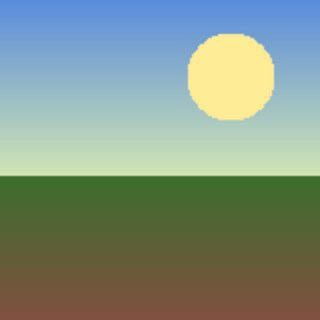
\includegraphics[width=100pt]{photo-cmyk.jpg}};
  \node[anchor=south west, inner sep=0] at (300,250) {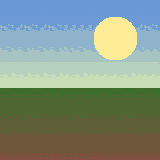
\includegraphics[width=100pt]{photo-indexed.png}};
  \node[anchor=south west, inner sep=0] at (420,250) {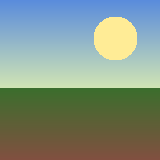
\includegraphics[width=100pt]{../pagecolor/photo.png}};

  % --- hairline rule like \hrule (0.4pt filled rect) ---
  \fill[black] (60,200) rectangle (520,200.4);
\end{tikzpicture}

% inline images (60x60pt) placed via TikZ nodes so their origin is exact
\begin{tikzpicture}[remember picture, overlay, x=1pt, y=1pt, shift={(current page.south west)}]
  \node[anchor=south west, inner sep=0, outer sep=0] at (60,120)
    {\pdfliteral direct{q 60 0 0 60 0 0 cm BI /W 1 /H 1 /CS /RGB /BPC 8 /F /AHx ID ff0000> EI Q}};
  \node[anchor=south west, inner sep=0, outer sep=0] at (180,120)
    {\pdfliteral direct{q 60 0 0 60 0 0 cm BI /W 1 /H 1 /CS /CMYK /BPC 8 /F /AHx ID ff000000> EI Q}};
\end{tikzpicture}

\clearpage

% ---------------------------------------------------------------- page 2: /Rotate 90
\pdfpageattr{/Rotate 90}
\noindent Rotated page (/Rotate 90).

\begin{tikzpicture}[remember picture, overlay, x=1pt, y=1pt, shift={(current page.south west)}]
  \fill[cmykred] (60,600)  rectangle (160,660);
  \fill[rgbblue] (180,600) rectangle (280,660);
  \node[anchor=base west, font=\Large, text=cmykred] at (60,560) {Rotated CMYK red node};
\end{tikzpicture}

\clearpage

% ---------------------------------------------------------------- page 3: offset CropBox
\pdfpageattr{/Rotate 0 /CropBox [50 50 400 600]}
\noindent CropBox [50 50 400 600].

\begin{tikzpicture}[remember picture, overlay, x=1pt, y=1pt, shift={(current page.south west)}]
  \fill[cmykred] (60,500)  rectangle (160,560);
  \fill[rgbblue] (180,500) rectangle (280,560);
  \node[anchor=base west, font=\Large, text=rgbblue] at (60,460) {Cropped RGB blue node};
\end{tikzpicture}

\end{document}
